\chapter{Methodology}\label{ch:methodology}


\section{Dataset}\label{sec:dataset}
The dataset was the same as in the unpublished study of Hammer et al~\cite{Hammer-2021}.
Modified with the authors permission, the description from~\cite{hammer-predominance-2016} of the experiment settings,
and the pre-processing follows.
It was not a part of this thesis to perform the modifications described below.
We were provided with the pre-processed dataset.

\subsection{Movement task and kinematic variables}\label{subsec:movement-task-and-kinematic-variables}
A dataset that was already successfully used in several other iEEG studies to examine decoding of movement kinematic parameters\cite{Hammer-2021,hammer-predominance-2016,hammer-role-2013} was utilized for the purposes of this thesis.
The participants performed a motor task consisting in a car-driving computer simulation.
They controlled the position of the car on a computer screen using a steering wheel which they held in both hands.
The task was to keep the car on a curved road.
The road was random without any repetitions, following a low-pass filtered white noise trajectory.
During the movement task, the position of the car on the road was measured.
The position of the car linearly corresponded to the deflection of the steering wheel and was measured relative to the screen center, which corresponded to zero-deflection of the steering wheel.
Importantly, the control of the car's position was possible only in the horizontal dimension (left - right).
The upward movements of the car (vertical scrolling speed) were kept constant in each run of the game and adjusted for each subject individually.

The difficulty and the recording time of each subject was also adjusted based on the participant's motivation/ability to participate, lasting $25 \pm 7$ min ($mean \pm SD$).
The car game difficulty was modified by the vertical scrolling speed of the car.
Therefore, to account for faster movements, the low-pass cutoff frequency was set to 10 Hz for smoothing the raw tracker data prior to the derivation of the kinematic parameters.
From the horizontal, 1-D trajectory, the following two kinematic parameters were derived:
1. velocity computed as a derivative of position, 2. speed as the absolute value of velocity.
Velocity thus contained the directional information in its sign;
for example, velocity values smaller than zero implicated movement to the left and vice versa, while speed indicated how fast the car was moving left or right (irrespective of its direction).
The time-series of the kinematic parameters were resampled at 250 Hz and temporally aligned to the iEEG data.

\subsection{Recording}\label{subsec:recording}
The recordings were performed in the University Medical Centre in Freiburg, Germany and in the Motol University Hospital in Prague, Czech Republic.
The study included 12 epilepsy patients (6 male, age 19--50, mean = 33, SD = 10) all of which had intracranial EEG implantations.
Some of the implantations were placed in the region of the motor cortex.
The location of the electrodes was dependent solely on the needs for medical evaluation of their medication-resistant epilepsy.
Both sEEG and ECoG electrodes were present among patients.
Detailed information about electrode type and placement is presented in Table\ref{tab:patient-table} and Figure\ref{fig:electrodes}.

\begin{figure}[!htbp]
\centering
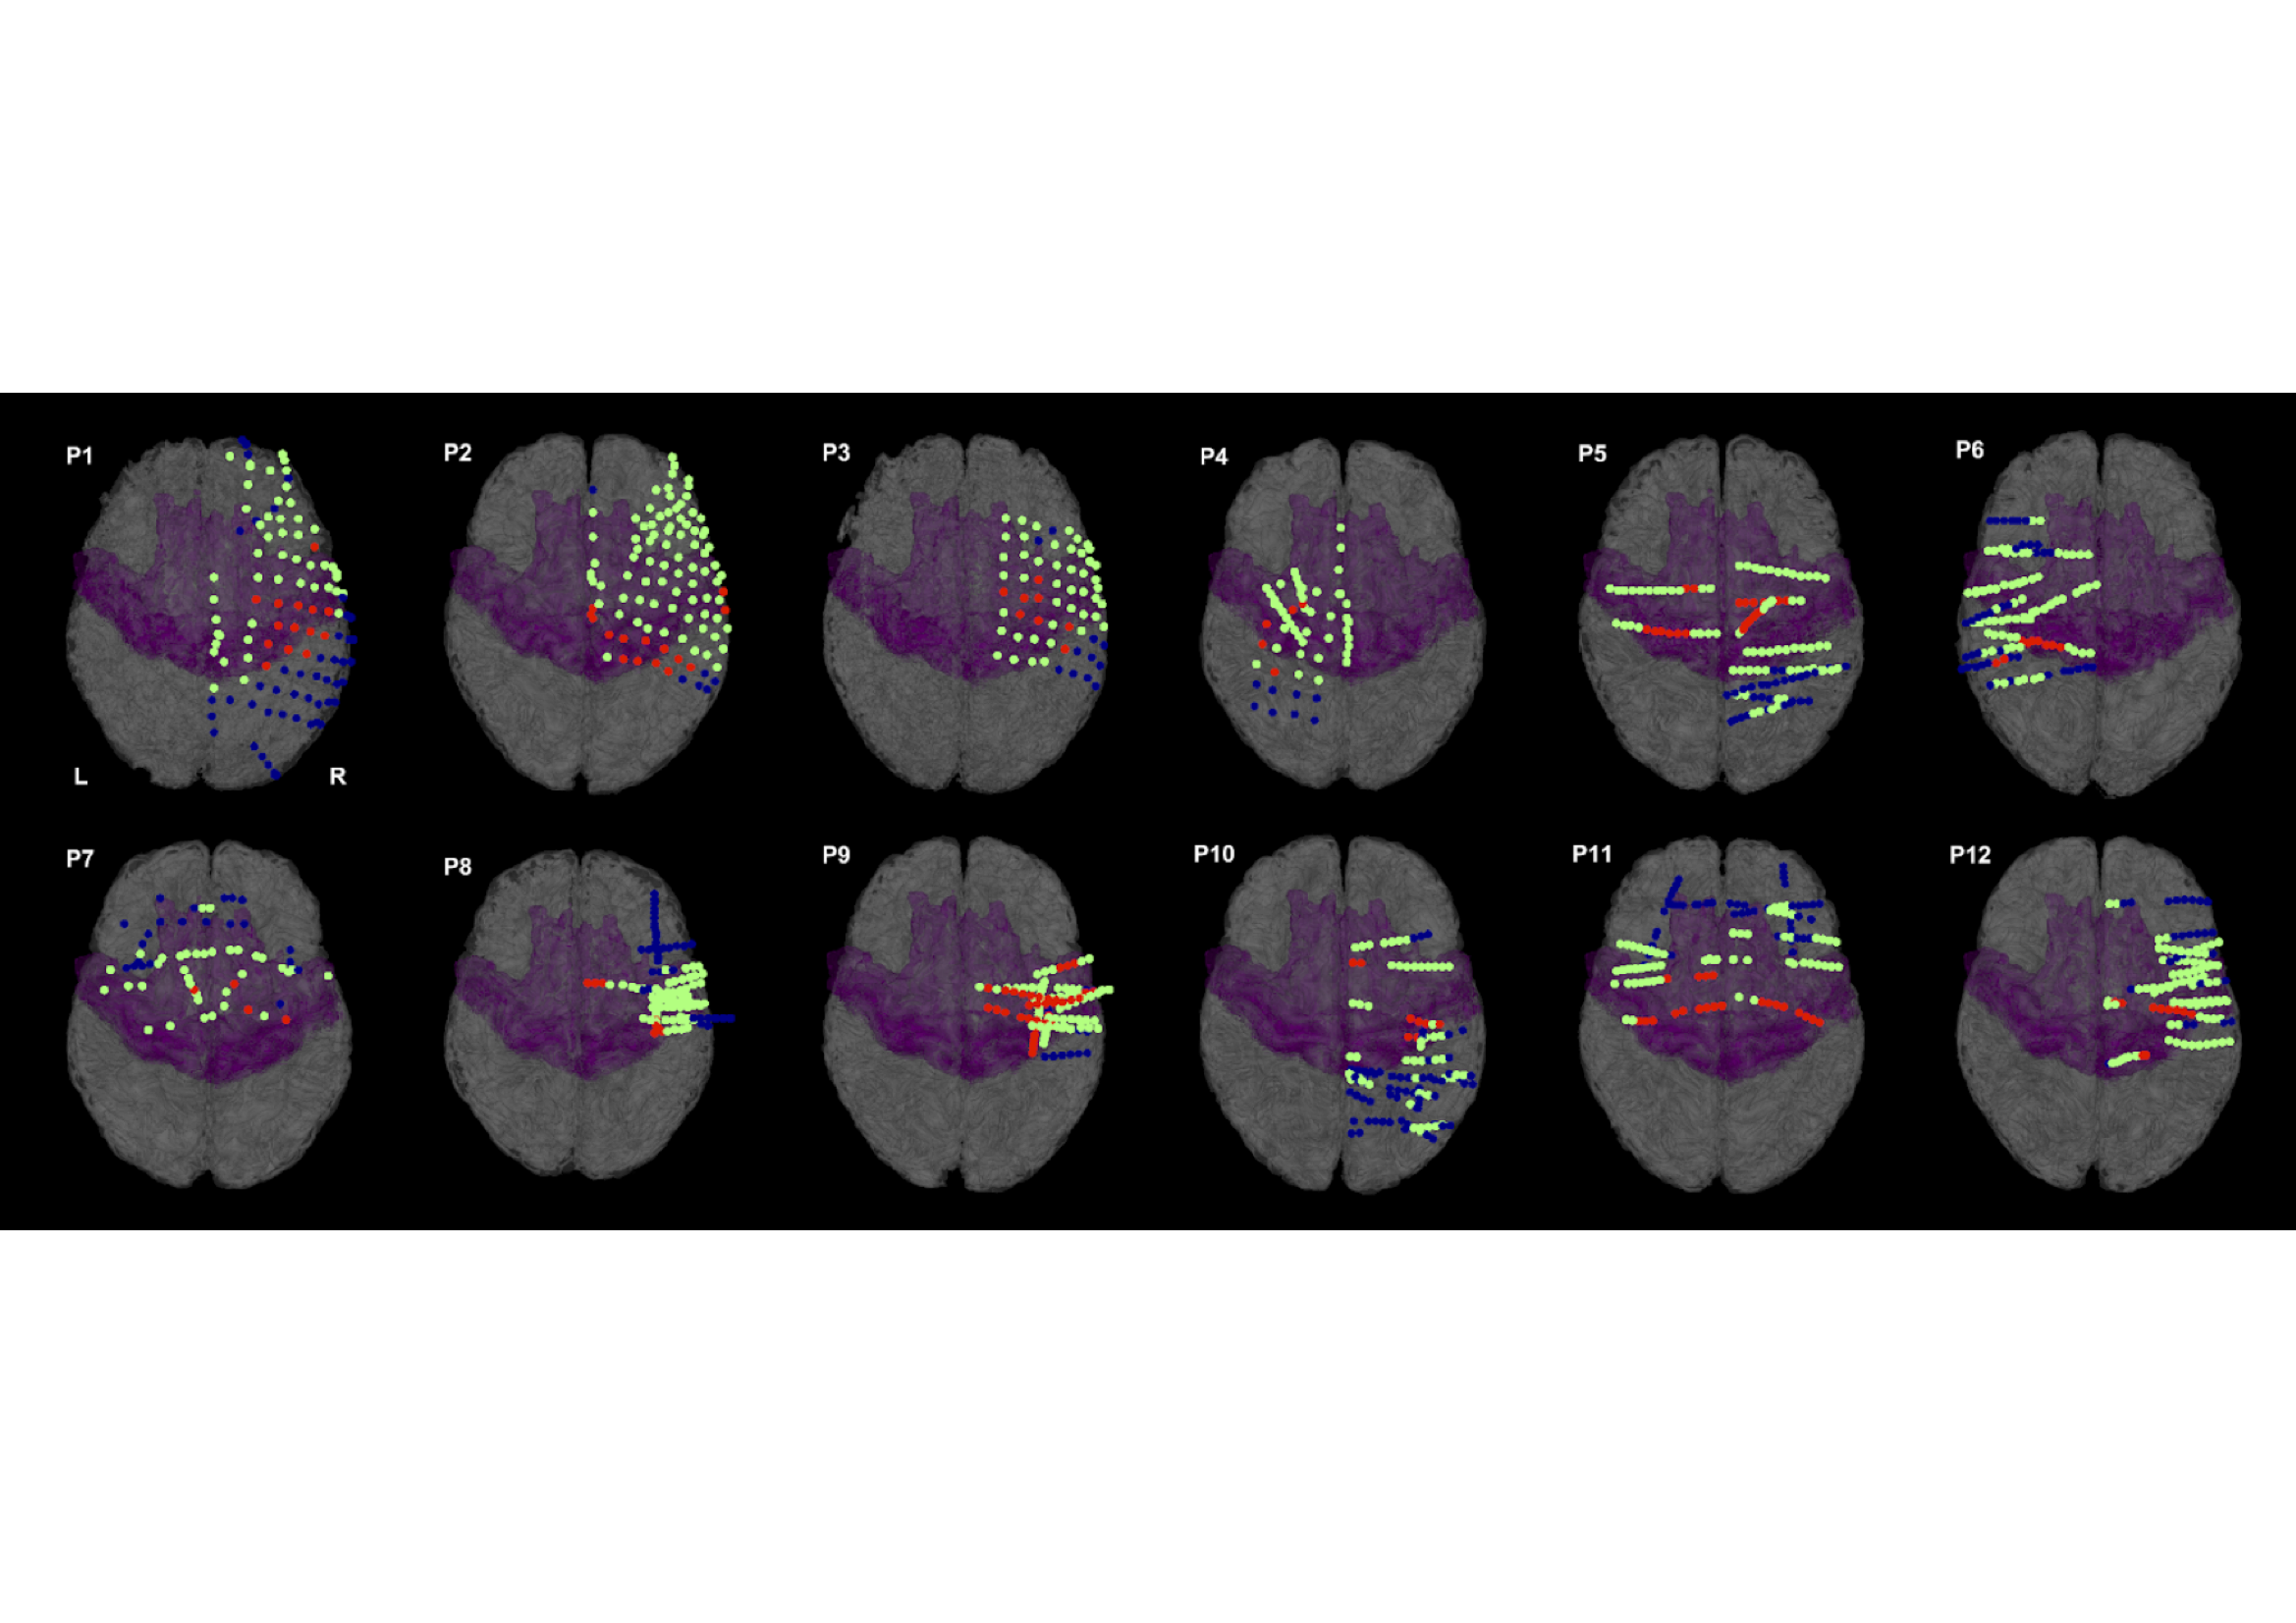
\includegraphics[width=0.8\linewidth]{img/ch3/electrodes}
\caption{}
\label{fig:electrodes}
\end{figure}

\begin{table}[!htbp]
\centering
\begin{tabular}{|p{1.3cm}|p{1.05cm}|p{2.15cm}|p{2.2cm}|p{2.2cm}|p{0.5cm}|p{0.65cm}|p{0.6cm}|p{0.8cm}}
\toprule
Patient & Sex (Age) & Pathology & Implant loc & Electrode type ($N$) & $N_r$ & $N_{ch}$ & $N_{m}$ & $N_{nm}$ \\
\midrule
P1 & F (47) & Cryptogenic & Right frontal & ECoG (98), intracerebral (12) & 25 & 85 & 14 & 47 \\
\hline
P2 & M (48) & FCD & Right fronto-temporal & ECoG (90), intracerebral (12) & 53 & 49 & 15 & 11 \\
\hline
P3 & M (50) & Cryptogenic & Right frontal & ECoG (64) & 3 & 61 & 8 & 11 \\
\hline
P4 & F (22) & FCD & Left frontal & ECoG (40), Intracerebral (12) & 11 & 47 & 5 & 16 \\
\hline
P5 & F (29) & Gilosis & Left and right fronto-parietal & Intracerebral (125) & 10 & 115 & 23 & 29 \\
\hline
P6 & M (29) & FCD & Left frontal & Intracerebral (125) & 34 & 91 & 9 & 39 \\
\hline
P7 & F (32) & FCD & Left and right insular & Intracelebral (61) & 14 & 47 & 4 & 22 \\
\hline
P8 & M (19) & FCD & Right insular & Intracerebral (117) & 16 & 101 & 9 & 36 \\
\hline
P9 & F (25) & Gliosis & Right insular & Intracerebral (117) & 21 & 96 & 35 & 12 \\
\hline
P10 & M (34) & FCD & Right fronto-parietal & Intracerebral (125) & 23 & 102 & 8 & 63 \\
\hline
P11 & M (34) & FCD & Left and right frontal & Intracerebral (126) & 11 & 115 & 21 & 48 \\
\hline
P12 & M (28) & Not operated & Right frontal & Intracerebral (125) & 20 & 105 & 10 & 27 \\
\bottomrule
\end{tabular}\label{tab:table}
\caption{Patients. $N_r$, $N_{ch}$, $N_{m}$, $N_{nm}$  : number of rejected, non-reject, hand-motor, and non-motor channels, respectively. FCD: focal cortical dysplasia.}
\label{tab:patient-table}
\end{table}

\subsection{Separation of motor and non-motor channels}\label{subsec:separation-of-motor-and-non-motor-channels}
A specific aim in the study of Hammer et al.\cite{Hammer-2021} was to show what the CNNs learned from the raw brain signals.
The hypothesis was that the CNNs would focus on information from the hand-motor cortex when solving a movement-related task.
To verify this hypothesis, the recorded channels were divided into two distinct, non-overlapping groups: 1. hand-motor channels and 2. non-motor channels.
The hand-motor channels induced a clear hand motor response after the electrical stimulation at low intensities underneath or around the electrode contacts.
The non-motor channels, on the other hand, produced no sensory/motor response after the stimulation.
Furthermore, a requirement of at least 1 cm distance from the motor and premotor areas (i.e. Area 4a, Area 4p and Area 6 from the SPM Anatomy toolbox\cite{eickhoff-new-2005}) had to be satisfied for a channel to be included in the non-motor group.
To this end, all MRI brain scans (T1-weighted sequence) were normalized to the MNI space and the electrodes' coordinates were read out from either the post-implantation MRI or CT scans53.
The average number of hand-motor channels was $13 \pm 9$ ($mean \pm SD$), while there were $29 \pm 18$ ($mean \pm SD$) non-motor channels.
Some electrodes did not fall into either of the hand-motor and non-motor channel groups (e.g. channels in the motor cortex the electrical stimulation of which induced leg-motor response).
These electrodes were then left out in some analysis, because the aim was to delineate the difference between the two distinct groups of channels (the hand-motor channel group and the non-motor channel group clearly far away from the motor cortex).


\subsection{IEEG data preprocessing}\label{subsec:ieeg-data-preprocessing}
The iEEG data preprocessing was also the same as in~\cite{Hammer-2021}.
A comprehensive rejection of \textit{epileptic} channels based on the information from the respective epilepsy centers was performed, because the primary aim was to investigate the physiological brain activity.
Thus, the channels, i.e. those located in the seizure onset zone and/or containing a large number of inter-ictal epileptiform discharges, were rejected from this study ($20 \pm 13$, $mean \pm SD$ over subjects Table\ref{tab:patient-table}).
All non-rejected iEEG channels ($85 \pm 28, mean \pm SD$) were referenced to their common average, high-pass filtered at 0.15 Hz (3rd order Butterworth filter), normalized to the inter-quartile range of each channel, and resampled to 250 Hz, to yield consistent data sets from the different recording systems used at both aforementioned epilepsy centers.
The iEEG data were resampled to 250 Hz in order to emulate the same setup of the Deep4Net from~\cite{schirrmeister-deep-2017}, which was successfully applied to demonstrate high-gamma (70 - 90 Hz) effects in decoding motor behaviour from non-invasive EEG. Importantly, any over-fitting in the preprocessing was carefully avoided (i.e., all parameters of the preprocessing of the test set were estimated on the training set) and only accusal, finite impulse response filters were applied.
Therefore, the decoding approach could be readily applied also in a closed-loop, online BMI.

The aligned iEEG and kinematic time-series were divided into 25-s long data segments.
In order to minimize a potential influence of temporal correlations in neighbouring data parts, the segments had a 2-s margins in between each other. Additionally, the last two minutes of the recordings were left as a test set. The evaluation test set was not a part of the dataset that was utilized in this thesis.

\subsection{Modifications to the dataset}\label{subsec:modifications-to-the-dataset}
In the scope of this thesis, we refer to multiple datasets which all are variations of the original dataset provided by the Motol University Hospital.
We performed the modifications to see how the network's performance/gradients change.
The modifications were of the three following types: 1. filtering of certain frequencies, 2. shifting the predicted time-point with respect to the input window, 3. spectral whitening.
\begin{itemize}
\item \textbf{Filtering} We created two types of datasets using filtering.
A high-pass filtered dataset using a 15th order Butterworth filter, cut-off frequency 60Hz, non-zero phase shift and a low-pass dataset using Butterworth filter order 15, cut-off frequency 60Hz, nonz-zero phase shift.
Besides full training on these datasets, parts of these datasets were combined for training and validation to see for example, how a network trained on full data performs on high-passed data etc.\\
The name of the model includes information about the data the model was trained on.
For example if a model name contains full-low it was trained on full data and validated on low-passed data.
If it contains high-high it was both trained and validated on high-passed data.

\item \textbf{Shifting} Originally in Hammer et al.~\cite{Hammer-2021} the network was constructed so that the predictions were made from signals recorded prior to their execution.
Besides using this, we also created a dataset which shifted the predicted time-point to the middle of the input window that is used for its prediction.
Such a dataset is not suitable for training a network suitable for online BCI since half of the input window is recorded after movement execution and therefore in the future with respect to what is being predicted.
Nevertheless, we were interested in what the shifting does to performance and the gradients.


\item \textbf{Spectral whitening} Lastly we also created whitened datasets.
Spectral whitening was performed so that amplitudes of all frequencies were normalized to one~\ref{fig:spectral-whitening}.
This was achieved using a Fourier transformation of each 25s long segment into the power spectrum, obtaining information about phase and amplitude.
Then dividing the amplitudes with their absolute value and then, via inverse Fourier transformation, transforming it back to signal.
The whitened signal was then iqr-normalized.
This normalization was calculated and applied to each segment on the training set and the same parameters averaged over all 25s long segments of the training set were applied to the validation set.

\begin{figure}[!htbp]
\centering
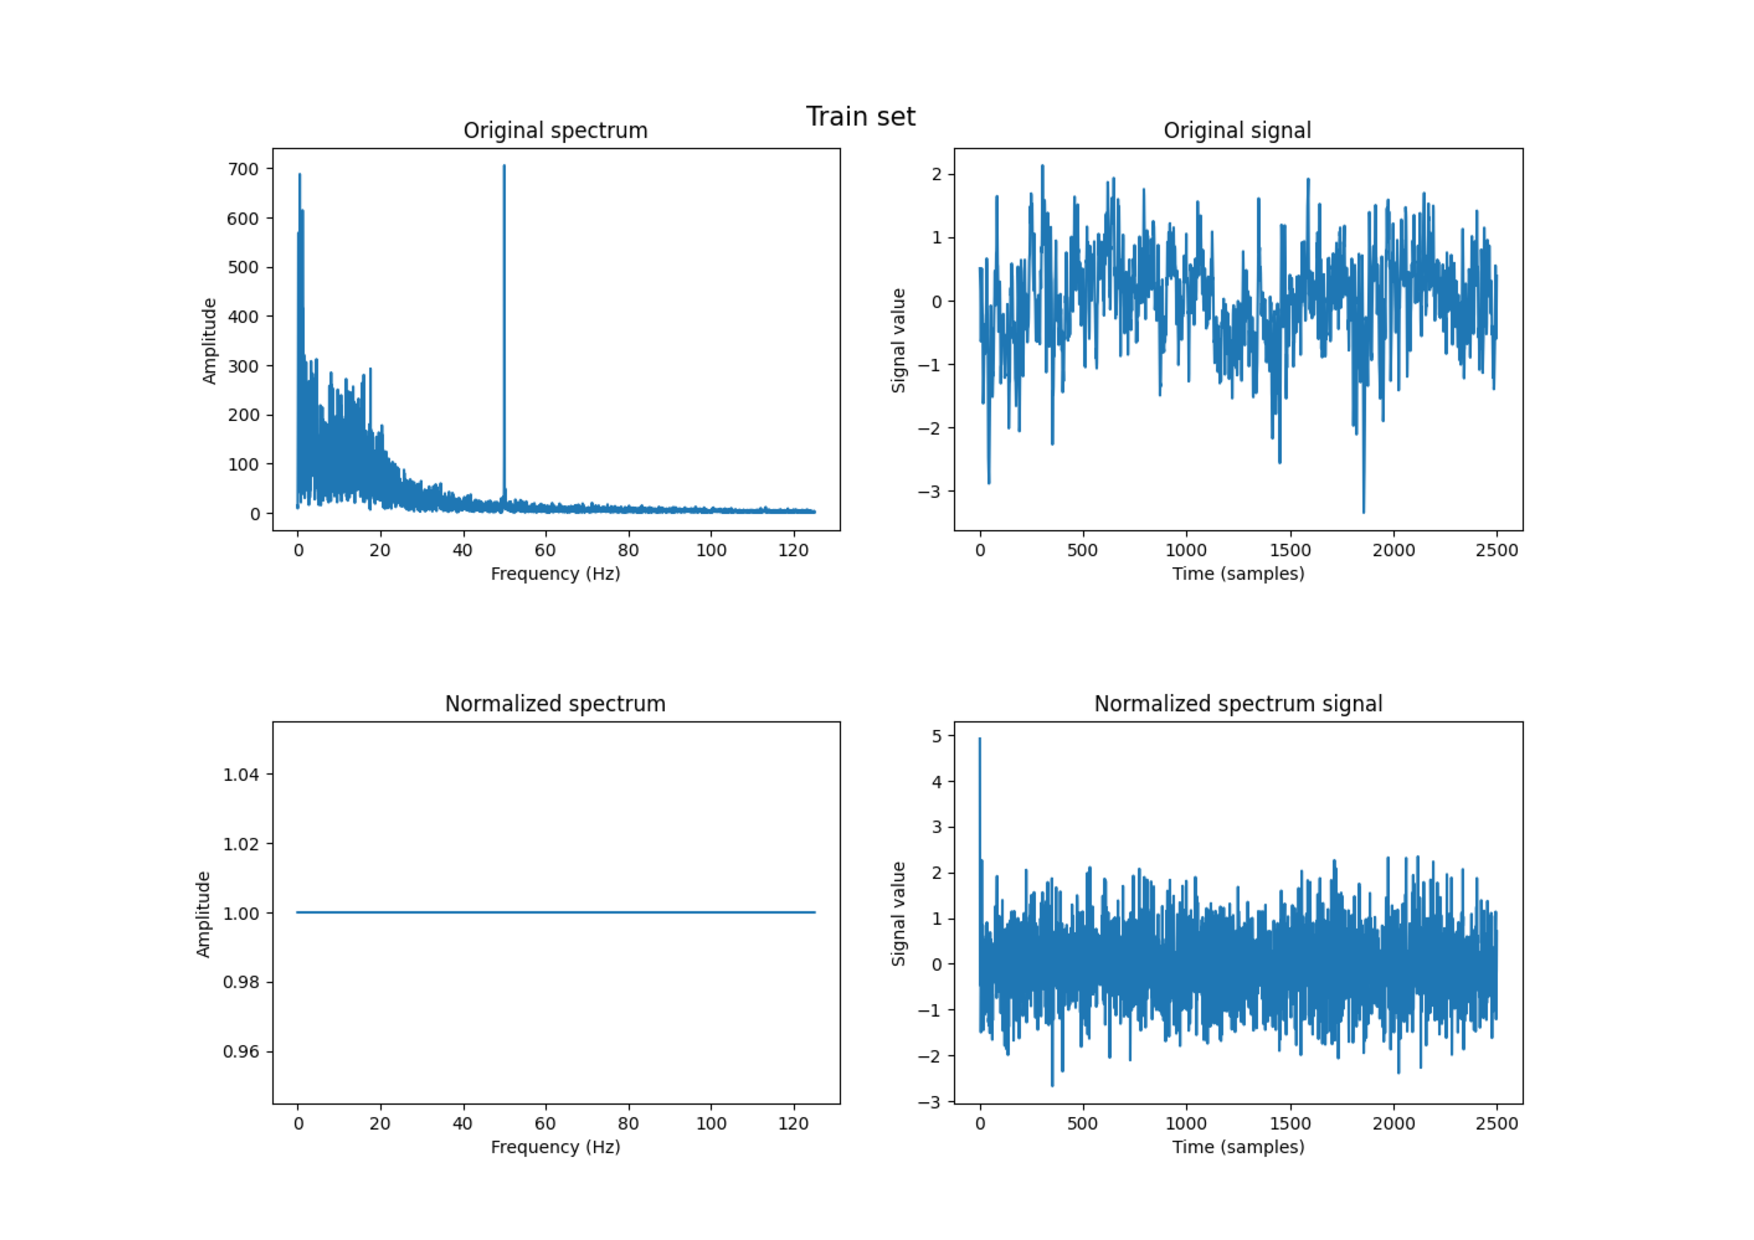
\includegraphics[width=\linewidth]{img/ch3/spectral-whitening}
\caption{The top row shows the original power spectrum of the iEEG signal and the original iEEG signals of the first 25s long segment.
The bottom row shows how spectral whitening changed both the spectrum and the signal.}
\label{fig:spectral-whitening}
\end{figure}
\end{itemize}

\section{Deep4Net}\label{sec:deep4net}
The Deep4Net, which is freely available in the Braindecode library, was already shortly described in Section~\ref{Background}.
In this section, we describe it in more detail together with the architectural changes that need to be made when cropped decoding is used and how it relates to the changes we were making to the architecture throughout our research. 
We also focus on how classification and regression differ and what it means with respect to the architecture, its inputs and outputs. 

\subsection{Architecture}\label{subsec:architecture}
The architecture which is available in the Braindecode library\footnote{https://braindecode.org} has been previously used in a number of EEG decoding tasks \cite{Hammer-2021, schirrmeister-deep-2017, hartmann-hierarchical-2018}.
It is implemented using PyTorch\footnote{https://pytorch.org}.
The input of the network is a 2D array with time-steps along one axis and channels along the other axis.
The architecture consists of four convolutional-max-pooling blocks and is designed so that a special first block can learn spatially global filters.
The following three standard blocks then allow for learning temporal hierarchies of local and global modulations~\cite{schirrmeister-deep-2017}.
The first convolutional block is split into two parts.
One performs convolution over time and the second over the channels with weights for all possible electrode pairs using filters of the preceding temporal convolution.
Because there is no activation function between these two layers, they could be merged, but the authors emphasize the regularization function of this separation because it forces a separation of the linear transformation into a temporal convolution and a spatial filter.
The convolutional blocks start with a convolutional layer, then a batch normalization layer follows, after which a non-linearity is added, in the case of the Deep4Net it is the exponential linear unit (ELU) function\cite{clevert-elu-2016}.
Finally a max-pool layer closes the convolutional block.
An output layer, which is a softmax, comes last.
To use this network for regression which is what we are doing in this thesis, the only modification that needs to be done is removing the last softmax layer.
The architecture already transformed for regression is depicted in Figure~\ref{fig:architecture}
Otherwise, no special measures have to be taken.
Nevertheless, the way the output is interpreted changes.
This is further described in Section~\ref{subsec:difference-between-deep4net-for-classification-and-regression} after we provide important context about cropped decoding.

\begin{figure}[!htbp]
\centering
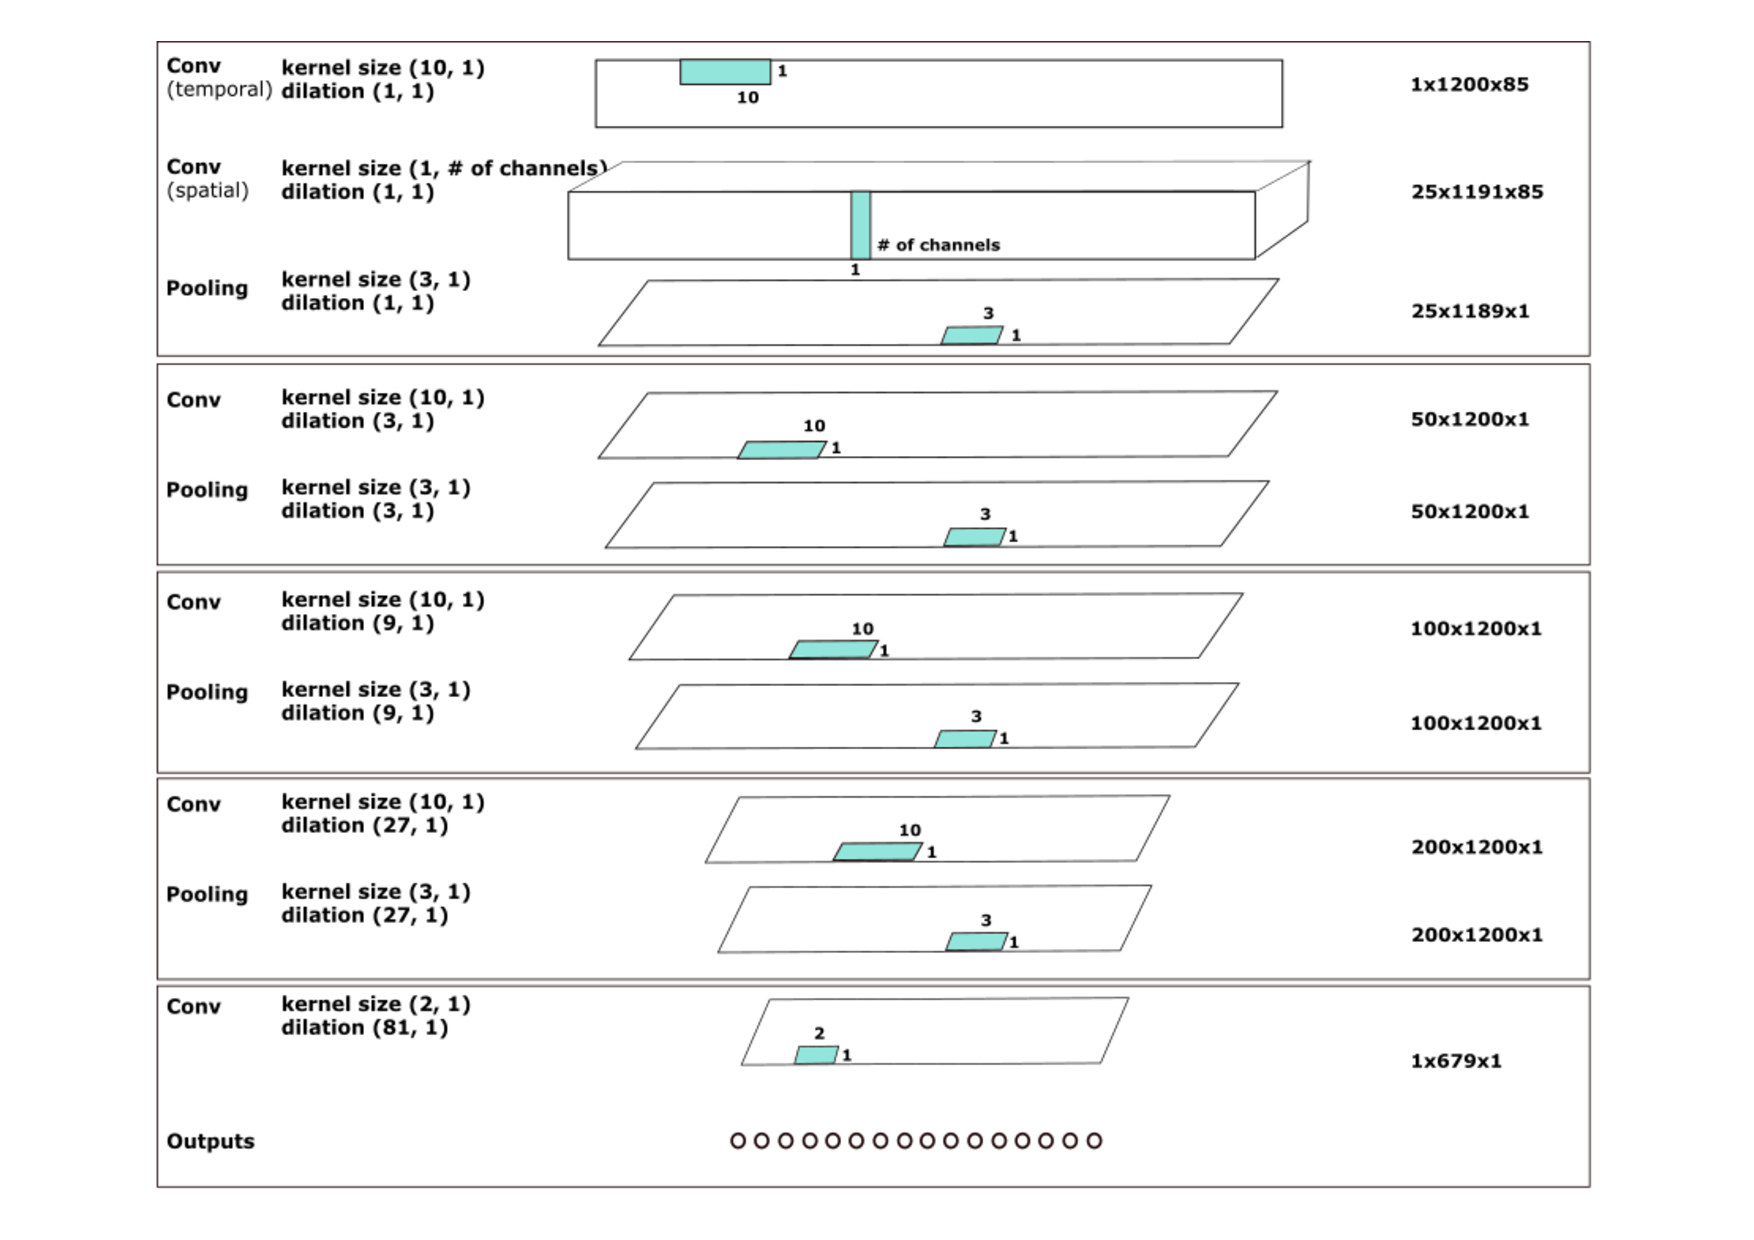
\includegraphics[width=\linewidth]{img/ch3/architektura}
\caption{The architecture of the Deep4Net modified to be suitable for regression.}
\label{fig:architecture}
\end{figure}

\subsection{Cropped decoding}\label{subsec:cropped-decoding}
Cropped decoding as implemented in~\cite{schirrmeister-deep-2017} augments the dataset.
Instead of giving one trial and obtaining one prediction, the trial window is separated into multiple smaller overlapping sub-windows each of which produce a prediction.
In case of classification, these multiple outputs for one input window are then averaged to give the final prediction from which loss is calculated Figure~\ref{fig:trial-wise-decoding}.
This way, the dataset is enlarged.

\begin{figure}[!htbp]
    \centering
    \RawFloats
    \begin{minipage}{0.4\textwidth}
        \centering
        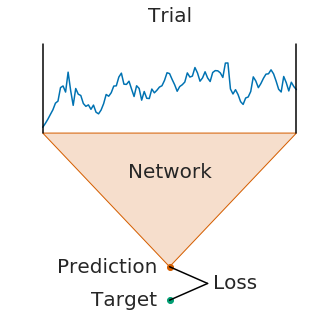
\includegraphics[width=0.9\textwidth]{img/ch3/trialwise-explanation}
        \caption{Trial-wise decoding - classification}
    \end{minipage}\hfill
    \begin{minipage}{0.5\textwidth}
        \centering
        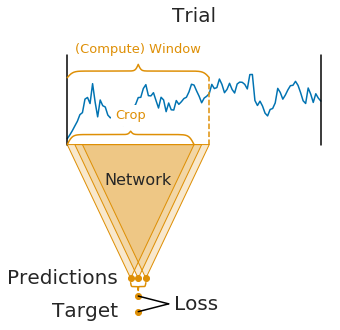
\includegraphics[width=0.9\textwidth]{img/ch3/trialwise-explanation2} 
        \caption{Cropped decoding - classification}
    \end{minipage}
\end{figure}\label{fig:trial-wise-decoding}


To avoid a longer training time, a trick with dilated convolution can be implemented.
This requires changes in the architecture.
In order to implement a network which can process multiple crops at the same time and give an equivalent result as the network processing one crop at a time, the strides of the layers can be removed (set to 1) and instead replaced by an increasing dilation.
The algorithm used to make the transition between strides and dilations is described in Algorithm\ref{alg:stride-to-dilation}.

Algorithm~\ref{alg:stride-to-dilation} describes how a network with stride is converted into a network with dilations.\\
\begin{algorithm}
\begin{lstlisting}[language=Python,label={lst:lstlisting}]
def to_dense_prediction(network):
	current_stride = 1
	for module in network.modules:
		if hasattr(module, 'dilation'):
			module.dilation = current_stride
		if hasattr(module, 'stride'):
			current_stride *= module.stride
			module.stride = 1
\end{lstlisting}
\caption{The simplified algorithm used to transform a network with strides to a network with dilations in the Braindecode library.
This version assumes a 1D stride and dilation which is sufficient for our case as all the strides in the networks are 1D.
}
\label{alg:stride-to-dilation}
\end{algorithm}

Importantly, this only works if the network has no padding or only left padding.
Right padding would disrupt the equivalency of computation.
The algorithm allows us to transform every network with stride and without right padding, into an equivalent network with dilations (dilated network).
Nevertheless, this relationship is not symmetric.
For some dilated networks no networks with strides performing an equivalent trial-wise computation exist.
An example of such a network is a network where in two consecutive layers with a dilation parameter, the first layer has bigger dilation than the second one.
This cannot happen if we follow the algorithm above~\ref{alg:stride-to-dilation} thus, such a network was not derived from a network with strides.

In Schirrmeister et al.~\cite{schirrmeister-deep-2017} the architectures were constructed in the space of the networks with stride and then converted into dilated networks.
This leaves a whole set of architectures unexplored.
Namely, those dilated networks which cannot be constructed from a network with stride.
It is important to point out that these dilated networks cannot be used for trial-wise decoding.
Nevertheless, as clearly follows from the next section~\ref{subsec:difference-between-deep4net-for-classification-and-regression}, this is no drawback for our task at hand.

\subsection{Difference between Deep4Net for classification and regression}\label{subsec:difference-between-deep4net-for-classification-and-regression}
We now describe the differences between using the Deep4Net for regression instead of classification.
In the classification task, one trial window was given as input having one gold label.
When using cropped decoding, the trial window was split into multiple shorter windows giving multiple outputs.
To get one output from these multiple outputs, the outputs were averaged to yield the final prediction.

In the case of regression we can also create an input window of a certain length and the label corresponding to it is the value of the kinematic variable at a certain time-point.
When we perform cropped decoding, we could just like for classification interpret all the outputs as belonging to the same prediction and averaging them.
But what Hammer et. al did, and also what we are implementing in this thesis, is interpreting each of these multiple outputs as consecutive values of the predicted variable which are directly used to calculate loss.
Therefore, there is no reason to perform trial-wise decoding and nothing prevents us from creating modified architectures for which it is impossible to create an equivalent network with strides.

The network is able to process varying input shapes.
It simply slides its convolutional filters over the input.
Therefore before training, the number of outputs needs to be calculated based on the size of the input window that was chosen.
The corresponding values of the predicted kinematic variables are cropped accordingly.
In this thesis, we used 1200 samples as input which corresponds to 4.8 seconds in time.
For the Deep4Net a window of 1200 samples gives 679 predictions.
Therefore, one prediction is made from $11200 - 679 + 1 = 522 $ samples measured before execution which translates to 2.088 seconds.
This is consistent with Hammer et al. where they used 2 second long segments.
Importantly to note, in Hammer et al. and also for the most part in this thesis, the input window predicting a time-point was shifted so that all the information used to decode this time-point happened prior to movement execution.
This makes the network suitable for online BCI\@.


\subsection{Receptive field}
The fact that the network cannot have right padding and in the case of the Deep4Net has no padding affects its receptive field.
By receptive field we mean the space of the input of the network which affects one specific output.
In \cref{fig:receptive-field} we visualize the receptive field for one prediction.
The figure illustrates how many times each input sample is used in computation throughout the pass through the CNN to obtain the specific prediction.
Note, that the receptive field in no way illustrates the weights of the network.

\begin{figure}[!htbp]
\centering
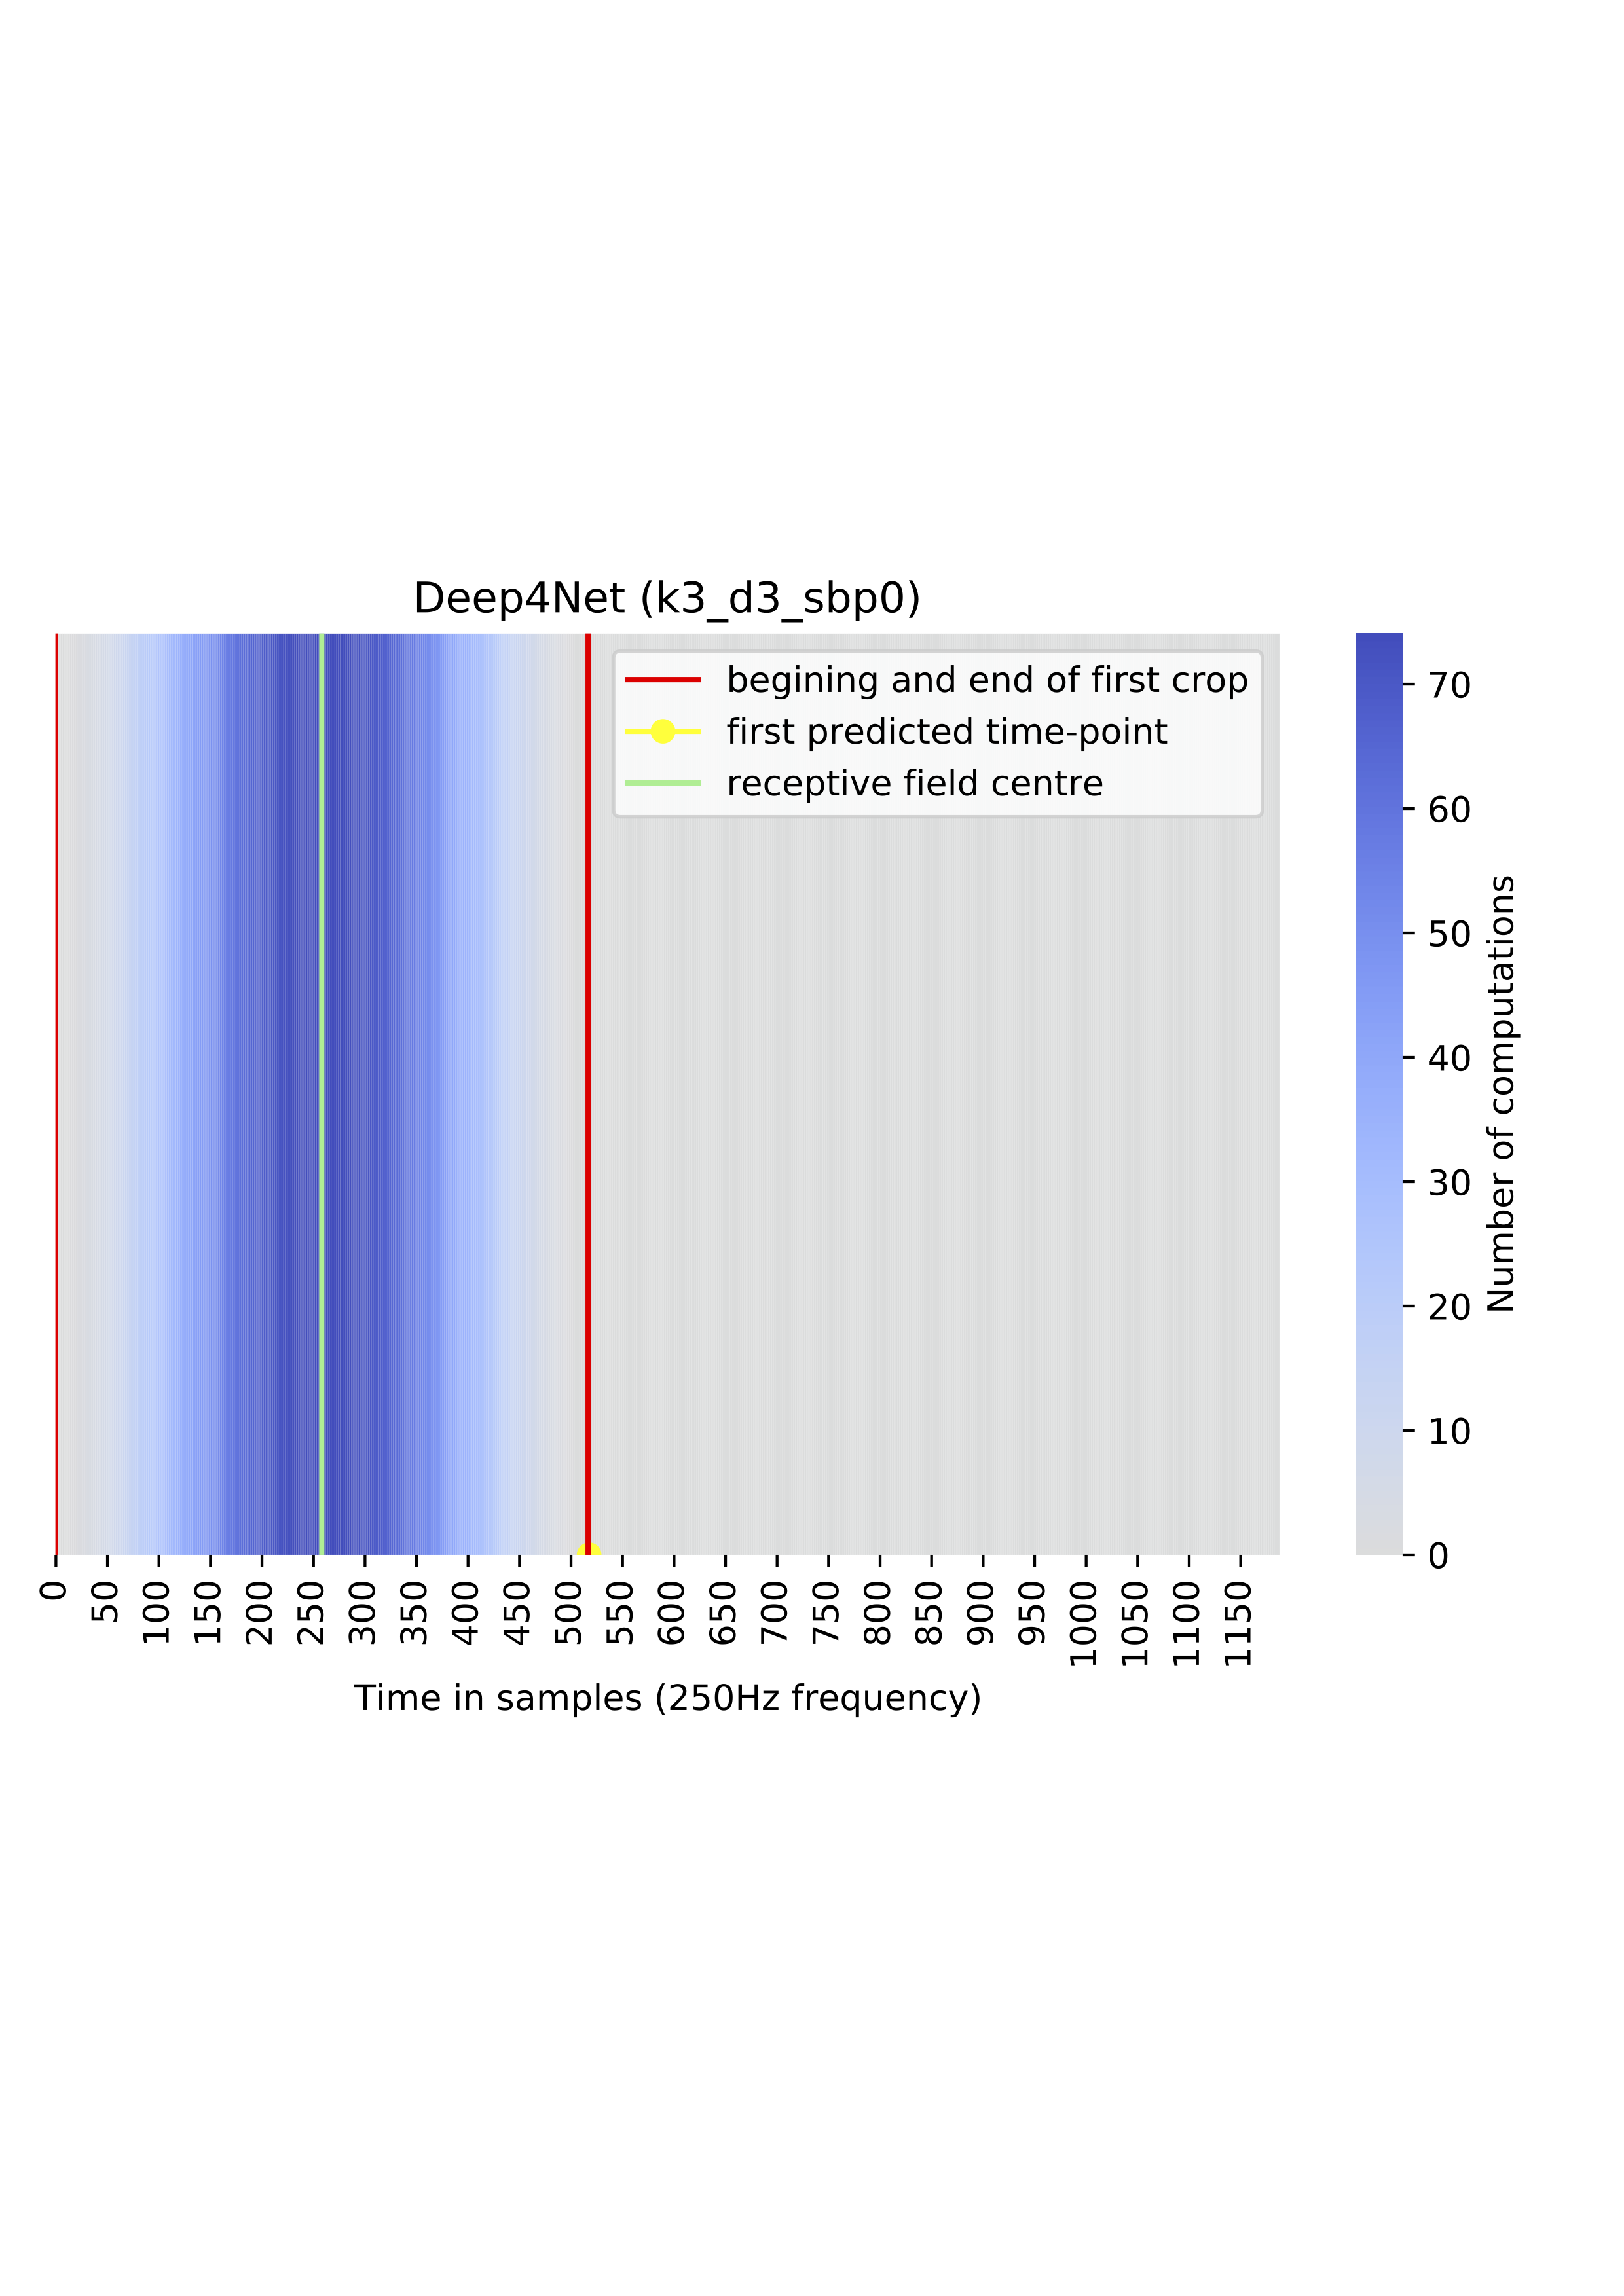
\includegraphics[width=0.8\linewidth]{img/ch3/deep4net-receptive-field}
\caption{The receptive field of the original Deep4Net, in this thesis denoted as {variable}\_k3\_d3\_sbp0. The vertical red lines delimit the first receptive field (crop) of the network used for calculating the first prediction. The green line represents the centre of the receptive field and the yellow dot on the x axis the first time-point that is being predicted. The gradient bar on the right shows the number of times each input sample was used in the calculations of the output.}
\label{fig:receptive-field}
\end{figure}

The receptive field is worthy of thought especially in the case of regression.
Figure \ref{fig:receptive-field} illustrates that the predicted time-point (red line) is fairly far from the centre of the receptive field (green line).
If we make the prediction only based on the data recorder prior to the predicted movement, the prediction is made from signals around the centre of the receptive field and the network pays little attention to the data that directly precede the movement.
For classification this is not as critical, because the same label is predicted from multiple crops, and the actual classified movement does not happen at the end of the last crop but at some point during the whole input window from which the crops are derived.
Therefore, the network has a chance to focus on information directly preceding the actual movement.
This change in the role of the receptive field between classification and regression might be a reason the network when employed to do regression does not use high-gamma.
The hypothesis here is, that the high-gamma signal is most informative directly before the movement execution.
Therefore, the distance of the network's receptive field centre to the predicted time-point hinders its usage.
We explore this in the \cref{sec:shifting-the-predicted-time-point}.

\subsection{Training}
Except for the learning rate, we left all hyper-parameters equal to those in Hammer et al., because it was our goal to reproduce their results and work from there.
The network was trained for 100 epochs with batch size 32, using Adam~\cite{kingma-adam-2017} as the optimizer and learning rate 0.001.
The reported learning rate in Hammer et al. was 0.01.
However, we used a lower learning rate because otherwise, the results were significantly worse than reported in Hammer et al.

For each patient separately, the 25s-long segments were divided into 5 equal or almost equal subsets and a 5-fold cross-validation was performed to estimate decoding accuracy.
The number of these segments varied among patients.
Therefore, the dataset sizes varied across models for different patients but the ratio was kept the same 80-20 training-validation.
In Hammer et.\ al, they performed leave-one-out cross-validation on the 25s-long segments.
Nevertheless, with the amount of different architecture and modified datasets we used, this would be extremely time consuming.
Therefore, we decided to do 5-fold cross-validation because it is also a good way of estimating the network's performance.

\subsection{Gradinet visualization}\label{subsec:gradinet-visualization}
In Schirrmeister et al. and Hammer et\ al. the main visualization method was input-perturbation output correlation.
However, after this method showed minor influence of high-gamma onto the network's prediction, they further investigated the network using gradient visualization.
The gradient visualization algorithm is the following.
First, the input signal is converted into the power spectrum using Fourier transformation.
After this transformation, hooks are created for the amplitude and phase values.
Then it is converted back into the original signal, this time using the torch functions so PyTorch can start building its computational graph reaching back to the amplitudes and phases.
This \textit{hooked} signal is then given to the network, whose weights are frozen, as input.
After obtaining the outputs, the outputs are averaged and the \texttt{torch.autograd.backward()} function is used to derive the gradients with respect to the frequency amplitudes and phases.

Throughout the thesis, the input window used in the above described algorithm was set to twice the size of the receptive field of the network to be consistent with \cite{Hammer_2021}.
A special case of the gradient visualization, namely when the input window was shortened so that the network had only one output was also explored as a part of this thesis.
In this special case, the outputs did not have to be averaged before using the \texttt{torch.autograd.backward()} function to derive the gradients.

To obtain representative gradients, the above described procedure is always repeated over multiple batches for each patient and the resulting gradients are averaged.
Because there are no significant differences between the gradients of the networks on the training set and the validation set we chose to always display the gradient values for the training set.
Also note that in this thesis we only address the gradients for the frequency amplitudes.
While inspecting the phase gradients would also be interesting, it is out of the scope of this thesis.


\subsection{Architerctural modifications}
Using the above described gradient visualization method, the group working on~\cite{Hammer-2021} found, that if the input window for the gradient visualization is set so, that the network only gives one output, and there is no averaging necessary before deriving the gradients, the graphs shows a big 83.33 Hz peak.
To inspect if this peak is an architectural artifact or not we performed a set of modifications to the architecture of the Deep4Net.
With our changes we focused on the kernel sizes and dilation parameters of the four max-pool layers present in the network.
Table~\ref{tab:architectures-description} explains the terminology used with respect to the max-pool parameters used throughout the thesis.
The original Deep4Net corresponds to the {variable}\_k3\_d3\_sbp0 in Table\ref{tab:architectures-description}.
The suffix \textit{sbp} refers to a parameter of the Deep4Net namely the \texttt{stride\_before\_pool} parameter.
This parameter influences the dilations in the max-pool layers of the network. In Hammer et al~\cite{Hammer-2021} and Schirrmeister et al. \cite{schirrmeister-deep-2017}this parameter was set to \texttt{False (sbp0)}, nevertheless, in the gradient peak analysis performed by their group which we are referring to in Section \cref{sec:gradient-peak}, the studied network had \texttt{stride\_before\_pool} set to \texttt{True (sbp1)}.
Therefore, we focus on the Deep4Net with sbp1 in the gradient peak analysis but the default Deep4Net architecture is the one with sbp0 as in Hammer et al.
When changing the parameters of the max-pool layers as we describe above, the number of outputs the network has changes.
It also causes changes in the receptive field of the network.
To see how, consider just one max-pool layer with dilation 3 (L3) and one max-pool layer with dilation 1 (L1). If we use a window of the same length as input for L3 and L1 and compare the dimensions of the outputs from these layers, the dimension of the output of L3 will be smaller than of the L1 \ref{figure_output_difference}.
Consequently, if we alter the dilation (and also kernel) parameters of the max-pool layers in the Deep4Net, we get a different number of outputs from the altered network.
When one network has dilations 1, 3, 9 and 27 in the max-pool layers (the k*\_d3) and the other one 1, 1, 1 and 1 (k*\_d1), the difference in the dimension of the output is significant.
The latter network makes more predictions from the same input length because the dimension of the output is larger.
It also has a smaller receptive field for one prediction as is visulalized in \cref{fig:receptive-field-comparison}.
Information about the size of the receptive field can also be found in Table\ref{tab:architectures-description}.


\begin{figure}
    \centering
    \RawFloats
    \begin{minipage}{0.45\textwidth}
        \centering
        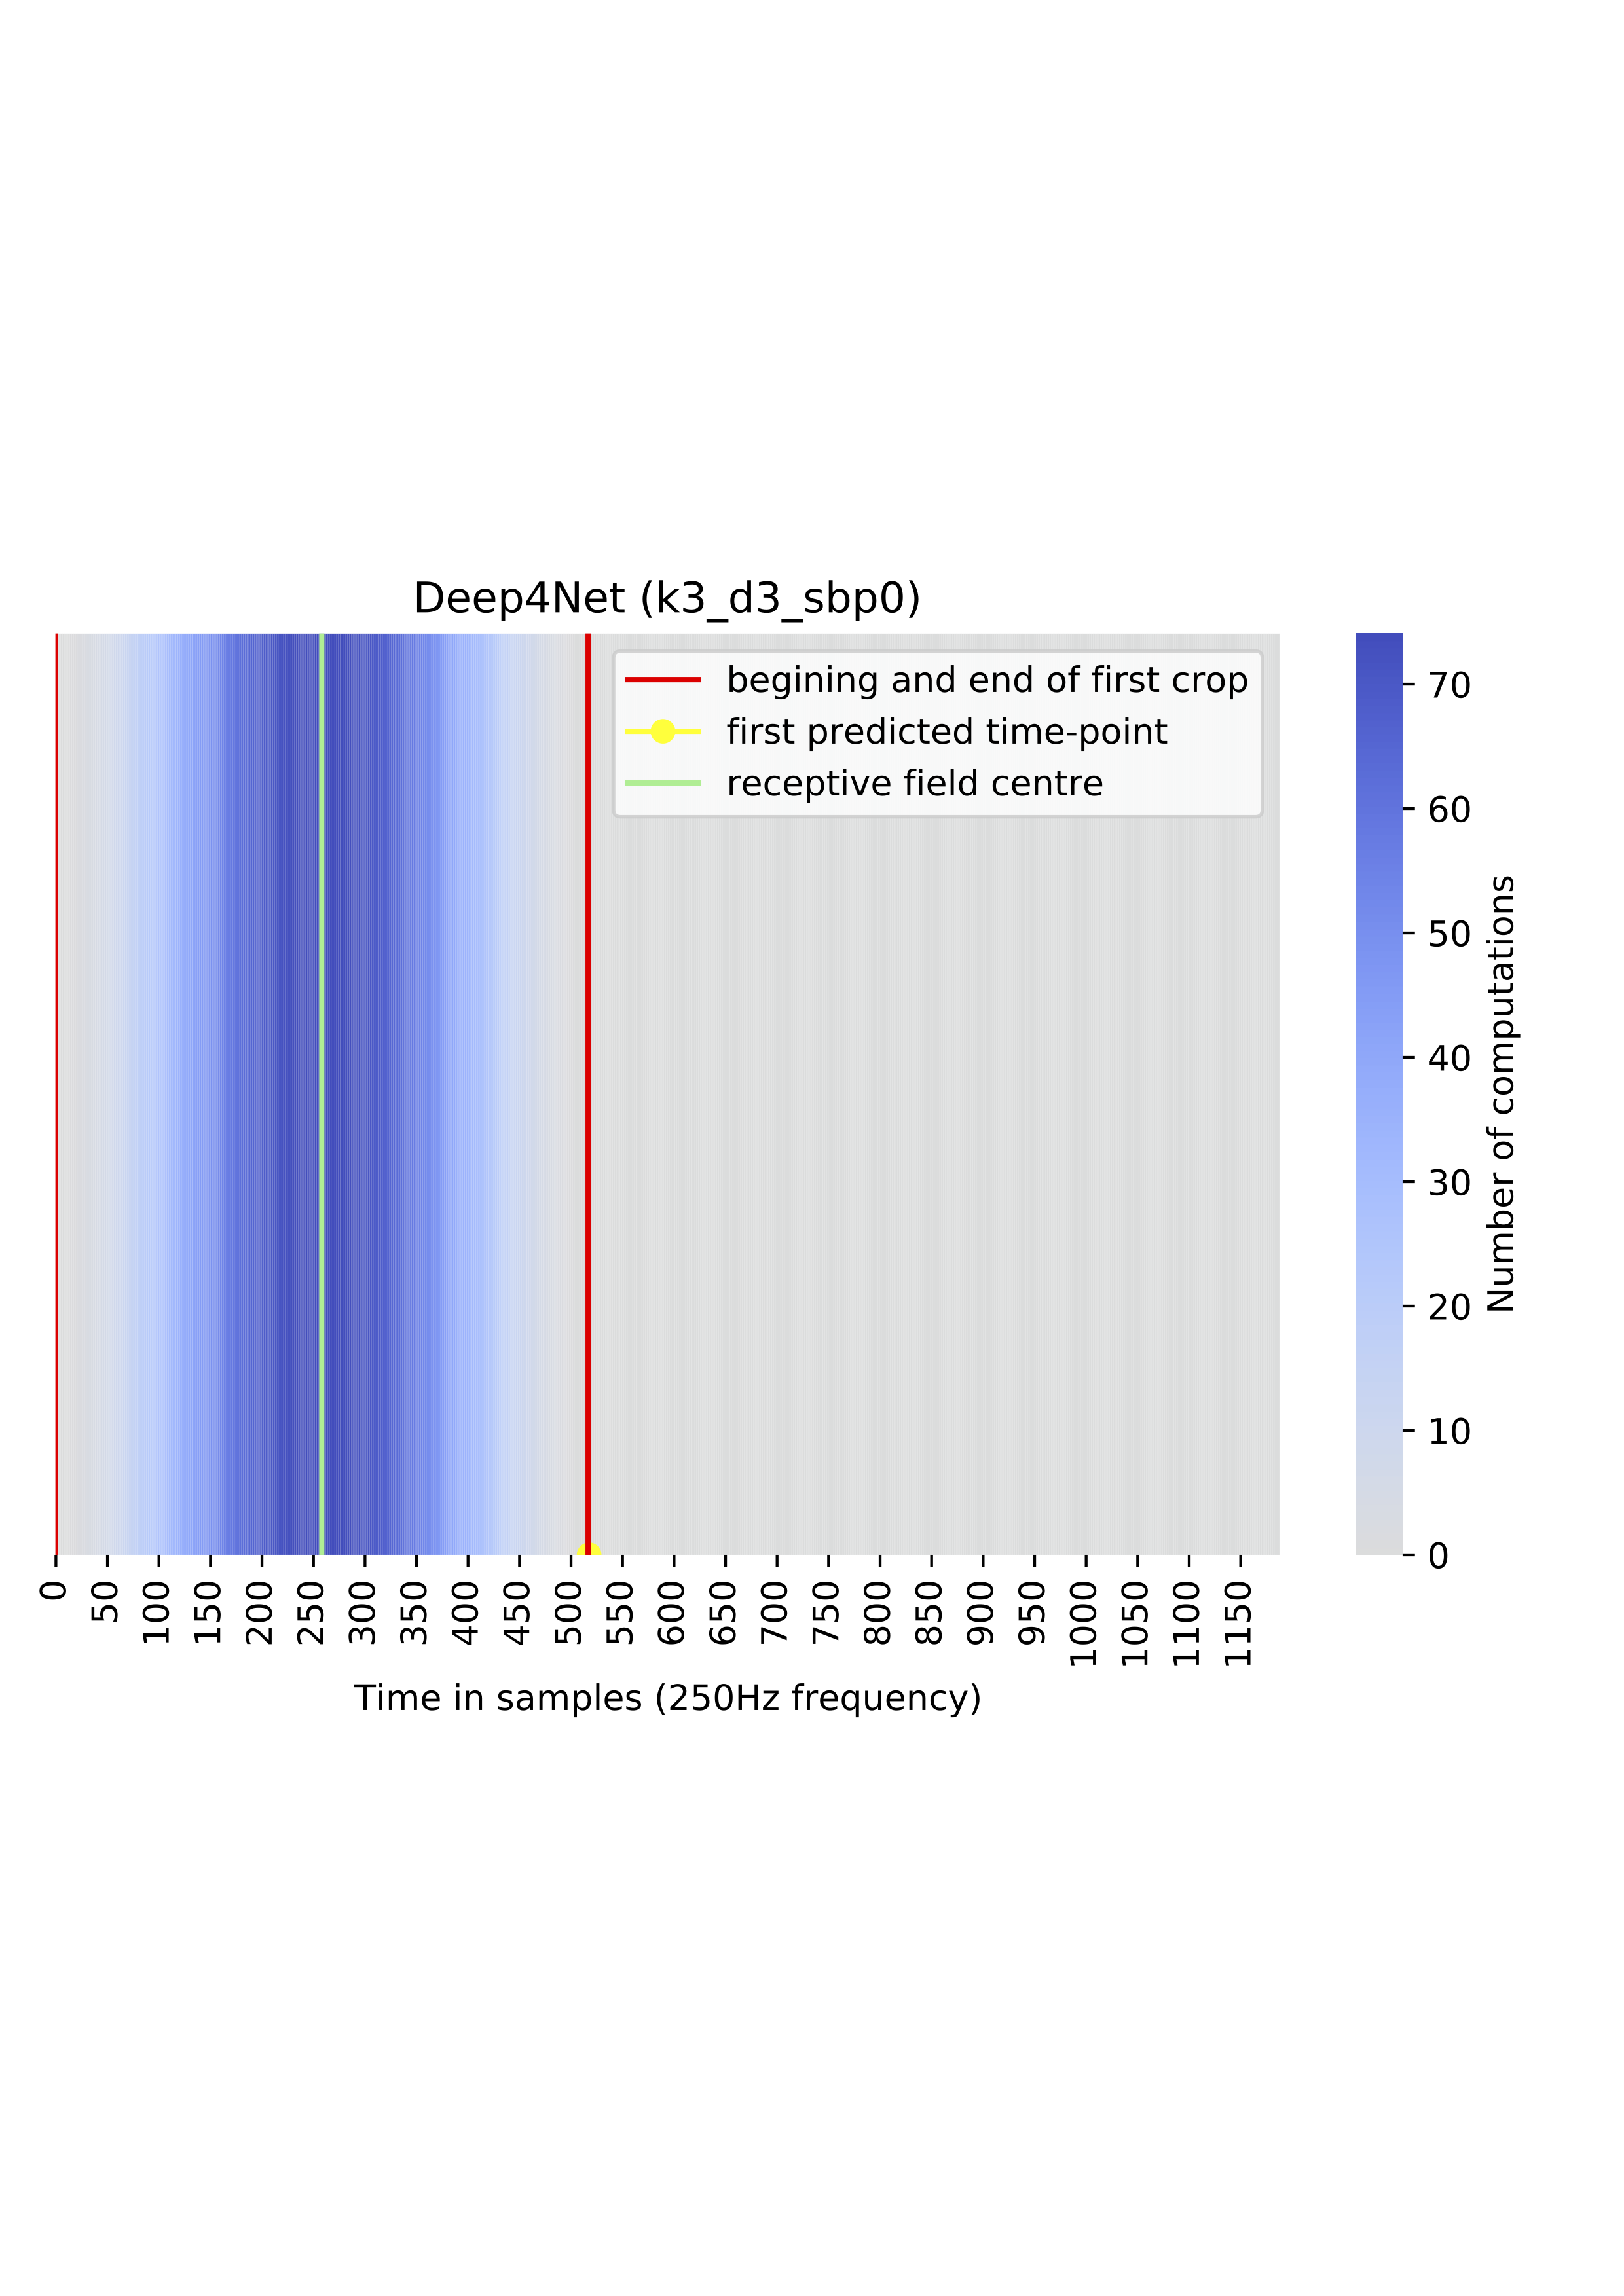
\includegraphics[width=0.9\textwidth]{img/ch3/deep4net-receptive-field} % first figure itself
        \caption{One example input window in which the receptive field of the network necessary for one prediction is highligted. In this case, the network is the Deep4Net.}
    \end{minipage}\hfill
    \begin{minipage}{0.45\textwidth}
        \centering
        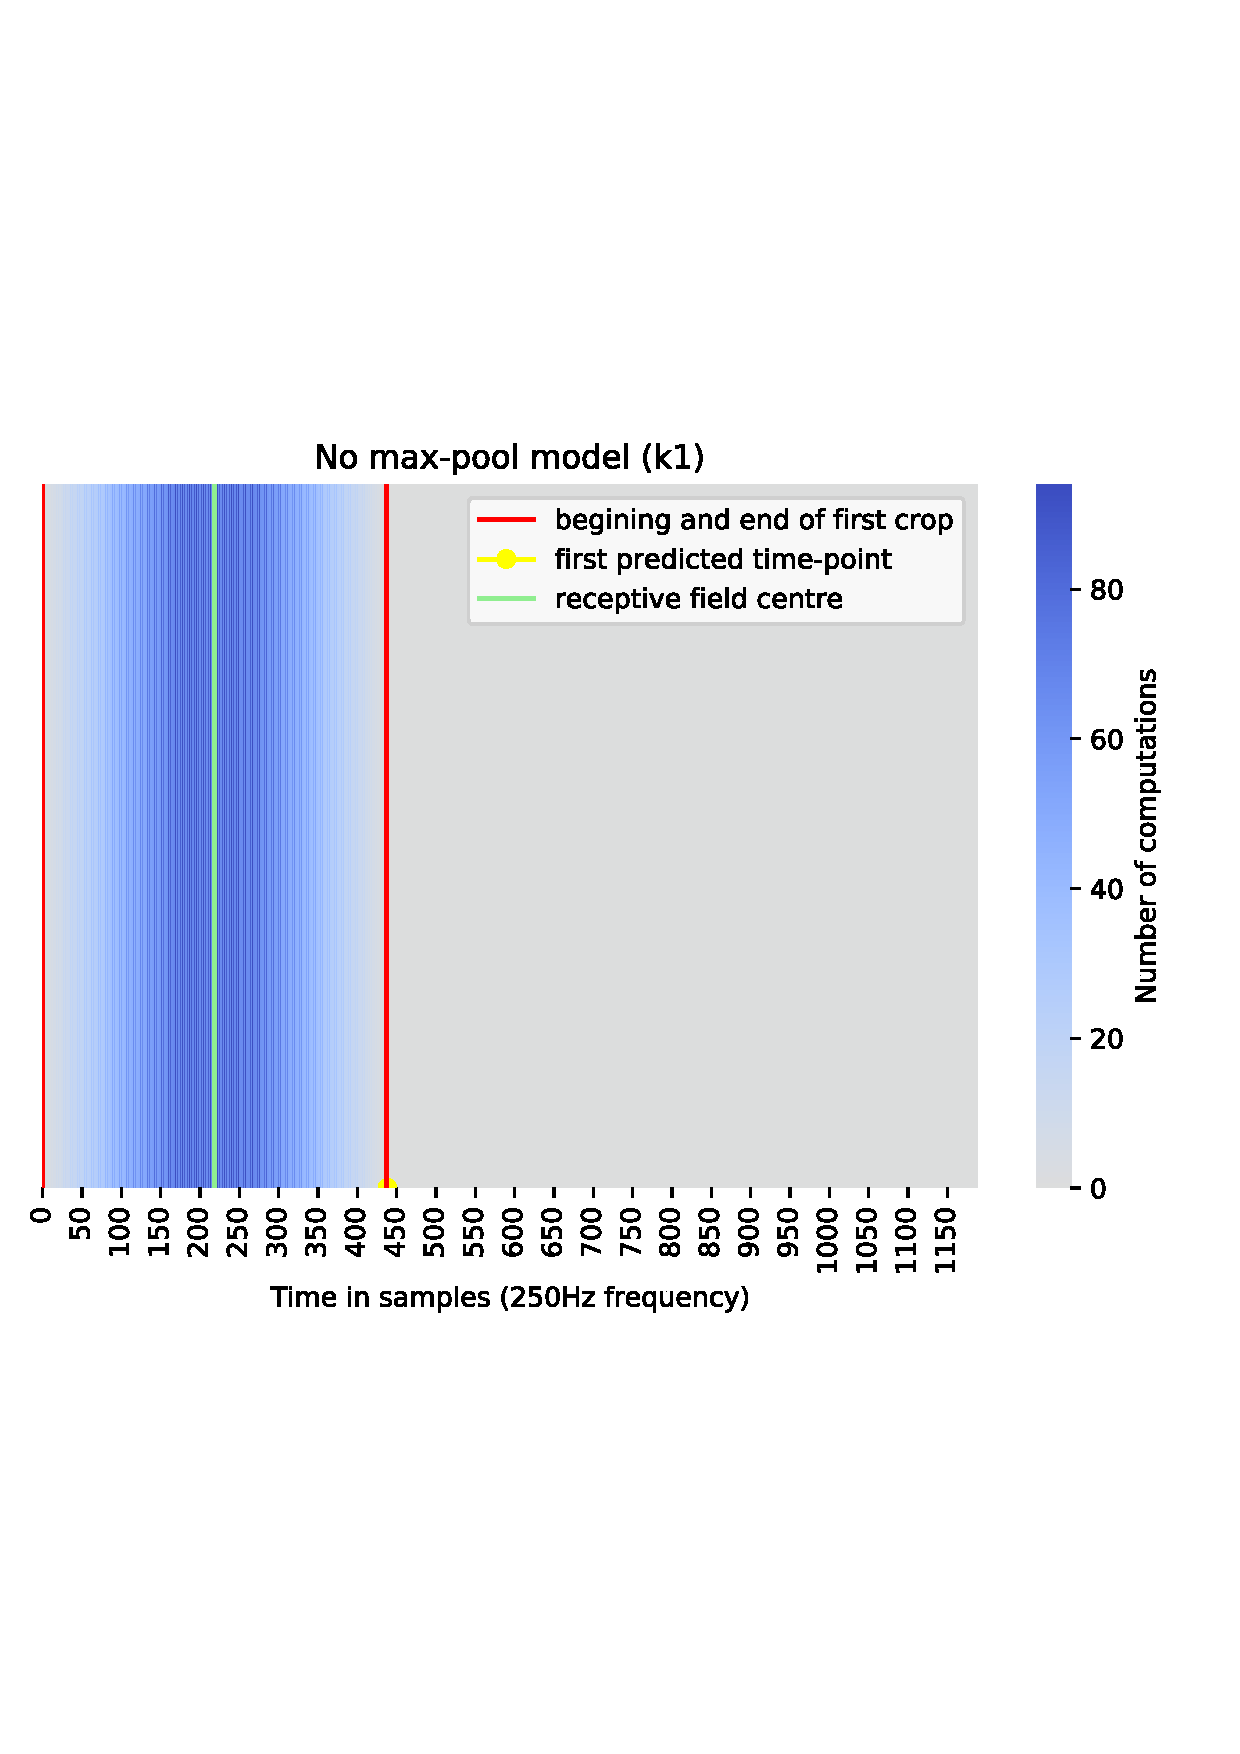
\includegraphics[width=0.9\textwidth]{img/ch3/k1-receptive-field} % second figure itself
        \caption{Network withtout max-pool.}
    \end{minipage}
\end{figure}\label{fig:receptive-field-comparison}



\begin{table}
\centering
\begin{tabular}{lllll}
\toprule
Model name & Max-pool kernel size & Max-pool dilations & Stride before pool & Size of the receptive field \\
\midrule
variable\_k1 & (1, 1), (1, 1), (1, 1), (1, 1) & No dilation & -- & 442 samples \\
\hline
variable\_k2\_d3 &(2, 1), (2, 1), (2, 1), (2, 1) & (3, 1), (9, 1), (27, 1), (81, 1) & -- & 562 samples \\
\hline
variable\_k3\_d3\_sbp1 & (3, 1), (3, 1), (3, 1), (3, 1) & (3, 1), (9, 1), (27, 1), (81, 1) & True & 682 samples \\
\hline
variable\_k3\_d3\_spb0 & (3, 1), (3, 1), (3, 1), (3, 1) & (1, 1), (3, 1), (9, 1), (27, 1) & False & 522 samples \\
\hline
variable\_k2\_d1 & (2, 1), (2, 1), (2, 1), (2, 1) & (1, 1), (1, 1), (1, 1), (1, 1) & -- & 446 samples \\
\hline
variable\_k3\_d1 &(3, 1), (3, 1), (3, 1), (3, 1) & (1, 1), (1, 1), (1, 1), (1, 1) & -- & 450 samples \\
\hline
variable\_k2\_d2 & (2, 1), (2, 1), (2, 1), (2, 1) & (2, 1), (4, 1), (8, 1), (16, 1) & -- & 472 samples \\
\hline
variable\_k3\_d2 &(3, 1), (3, 1), (3, 1), (3, 1)& (2, 1), (4, 1), (8, 1), (16, 1) & -- & 502 samples \\
\hline
\bottomrule
\end{tabular}
\caption{Architectural variations.}
\end{table}\label{tab:architectures-description}


\subsection{Performance analysis}
When comparing two models, we are not comparing them based on the mean-square error (MSE) which is the loss function of the training, but on the correlation coefficient (CC) between the model's predictions and the predicted kinematic variable.
Specifically the Pearson's correlation coefficient.
Often throughout the thesis we show boxplots of CCs of different architectures.
Each boxplot is obtained from performing a 5-fold cross-validation for each of the 12 participants.
The results from the 5 folds are averaged and the box-plot is created from the 12 averages.
While it is possible to create the box-plots from all the folds and not averaging them for each patient, we are interested in the distribution of correlation among patients rather than among individual runs.